% $Header: /Users/joseph/Documents/LaTeX/beamer/solutions/conference-talks/conference-ornate-20min.en.tex,v 90e850259b8b 2007/01/28 20:48:30 tantau $

\documentclass{beamer}

% This file is a solution template for:

% - Talk at a conference/colloquium.
% - Talk length is about 20min.
% - Style is ornate.



% Copyright 2004 by Till Tantau <tantau@users.sourceforge.net>.
%
% In principle, this file can be redistributed and/or modified under
% the terms of the GNU Public License, version 2.
%
% However, this file is supposed to be a template to be modified
% for your own needs. For this reason, if you use this file as a
% template and not specifically distribute it as part of a another
% package/program, I grant the extra permission to freely copy and
% modify this file as you see fit and even to delete this copyright
% notice. 

\usefonttheme{serif}
\usepackage{xcolor}% or package color

\mode<presentation>
{
  \usetheme{Warsaw}
  % or ...

  \setbeamertemplate{headline}{}
  
  \setbeamercovered{transparent}
  % or whatever (possibly just delete it)
}

\setbeamertemplate{footline}[frame number]
\setbeamertemplate{caption}[numbered]
\beamertemplatenavigationsymbolsempty

% or whatever

%\usepackage[utf8]{inputenc}
% or whatever

% \usepackage{times}
%\usepackage[T1]{fontenc}
% Or whatever. Note that the encoding and the font should match. If T1
% does not look nice, try deleting the line with the fontenc.

\usepackage[brazil]{babel}
\usepackage[utf8]{inputenc}
\usepackage[T1]{fontenc}
%\usepackage{subfigure}
\usepackage{amsmath,mathtools}
\usepackage{lmodern}			% for the fone to be bold and italic at the same time
\usepackage{tikz}
\usepackage{bigstrut}
\usepackage{pgfplots}
\usepackage{icomma}
\usepackage{graphicx}
\usepackage{epsfig}
\usepackage{subcaption}
\usetikzlibrary{positioning,arrows,shapes.geometric}
\usetikzlibrary{patterns}
%\usepackage{cite}
\usepackage[style=authoryear,backend=bibtex]{biblatex}
\addbibresource{../Referencias/referencias}
%\usepackage{color}
\usepackage{hyperref}
%\hypersetup{
%     colorlinks   = true,
%     allcolors    = blue,
%     citecolor = red,
%}
% \tikzstyle{int} = [draw, fill=blue!20, minimum size=2em]
% \tikzstyle{init} = [pin edge={to-,thin,black}] % end first type of initializations%
% \tikzstyle{block} = [draw, fill=blue!20, rectangle, rounded corners, 
%     minimum height=3em, minimum width=4em]
% \tikzstyle{sum} = [draw, fill=blue!20, circle, node distance=1cm]
% \tikzstyle{input} = [coordinate]
% \tikzstyle{output} = [coordinate]
% \tikzstyle{pinstyle} = [pin edge={to-,thin,black}]

\tikzstyle{decision} = [diamond, draw, fill=blue!20, 
    text width=4.5em, text badly centered, node distance=3cm, inner sep=0pt]
\tikzstyle{block} = [rectangle, draw, thick,%fill=blue!20, 
    text width=6em, text centered, rounded corners, minimum height=4em]
\tikzstyle{line} = [draw, -triangle 45]
\tikzstyle{cloud} = [draw, ellipse,fill=red!20, node distance=3cm,
    minimum height=2em]

\title[Simulated Humanoid Robot Control With Reinforcement Learning] % (optional, use only with long paper titles)
{Simulated Humanoid Robot Control With Reinforcement Learning}%{Decisão Automática de Duração de Passo de Caminhada Humanoide usando Programação Misto-inteira}

%\subtitle
%{Include Only If Paper Has a Subtitle}

\author % (optional, use only with lots of authors)
{Luis Guilherme G. Aguiar\inst{1}, Takashi Yoneyama \inst{1} e Marcos R. O. A. Maximo \inst{2}}
% - Give the names in the same order as the appear in the paper.
% - Use the \inst{?} command only if the authors have different
%   affiliation.

\institute[Instituto Tecnológico de Aeronáutica (ITA)] % (optional, but mostly needed)
{
\inst{1}%  \inst{2}%
  Divisão de Engenharia Eletrônica, Instituto Tecnológico de Aeronáutica (ITA) \\
\inst{2}%
  Laboratório de Sistemas Computacionais Autônomos (LAB-SCA), Divisão de Ciência da Computação (IEC), Instituto Tecnológico de Aeronáutica (ITA)
}
% - Use the \inst command only if there are several affiliations.
% - Keep it simple, no one is interested in your street address.

\date % (optional, should be abbreviation of conference name)
{Exame de Tese, 29/06/2018}
% - Either use conference name or its abbreviation.
% - Not really informative to the audience, more for people (including
%   yourself) who are reading the slides online

% \subject{Multi-agent Systems}
% This is only inserted into the PDF information catalog. Can be left
% out. 



% If you have a file called "university-logo-filename.xxx", where xxx
% is a graphic format that can be processed by latex or pdflatex,
% resp., then you can add a logo as follows:

\pgfdeclareimage[height=0.5cm]{university-logo}{figures/ita}
\logo{\pgfuseimage{university-logo}}


% Delete this, if you do not want the table of contents to pop up at
% the beginning of each subsection:
\AtBeginSection[]
{
  \begin{frame}<beamer>{Roteiro}
    \tableofcontents[currentsection]
  \end{frame}
}

% \AtBeginSubsection[]
% {
%   \begin{frame}<beamer>{Outline}
%     \tableofcontents[currentsection,currentsubsection]
%   \end{frame}
% }


% If you wish to uncover everything in a step-wise fashion, uncomment
% the following command: 

% \beamerdefaultoverlayspecification{<+->}


\begin{document}

\newcommand{\originalsystem}[1][]{ %1 optional param. for options of the tikz picture
\scalebox{0.8} {
	\begin{tikzpicture}[auto, node distance=3.5cm, scale = 0.9, every node/.style={transform shape}]
    		\node [input, name=input] {};
    		\node [block, right of=input] (system) {$f$};
    		\node [output, right of=system] (output) {};

    		\draw [draw,->] (input) -- node {$ \upsilon_2^i $} (system);
    		\draw [->] (system) -- node [name=y] {$ \dfrac{\partial{\tilde{\lambda}_2}}{\partial{p_i}} $}(output);
	
	\end{tikzpicture}
	}
}

\newcommand{\modifiedsystem}[1][]{
\scalebox{0.8} {
	\begin{tikzpicture}[auto, node distance=3.5 cm, scale = 0.9, every node/.style={transform shape}]     
		\node [input, name=input] {};
    		\node [block, right of=input] (system) {$f$};
    		\node [block, right of=system] (delay) {$\delta$};
    		\node [output, right of=delay] (output) {};

    		\draw [draw,->] (input) -- node {$ \upsilon_2^i $} (system);
   		\draw [->] (system) --node [name=y2] {$  $}(delay);
    		\draw [->] (delay) --node [name=y4] {$ \dfrac{\partial{\tilde{\lambda}_2}}{\partial{p_i}} $} (output);
	\end{tikzpicture}
	}
}

\definecolor{forestgreen}{rgb}{0.13, 0.55, 0.13}

\begin{frame}
  \titlepage
\end{frame}

\begin{frame}{Roteiro}
  \tableofcontents
  % You might wish to add the option [pausesections]
\end{frame}

% ================================================================================
\section{Introdução}

%\begin{frame}{Motivação}
%\begin{columns}[T] % align columns
%\begin{column}{.5\textwidth}
% \begin{itemize}
%  \item Locomoção por pernas é um dos problemas mais difíceis da Robótica Móvel.
%  \item Características de um problema difícil de controle: dinâmica não-linear, sub-atuada e com alta dimensionalidade.
%  \item Técnicas bem sucedidas usam modelos reduzidos de dinâmica.
% \end{itemize}
%\end{column}
%\begin{column}{.5\textwidth}
%  \begin{figure}[h!]
%   \centering
%       \includegraphics[width=0.8\textwidth]{Darwin_OP_6.jpg}
% \caption{Robô DARwIn-OP.}
% \end{figure}
%\end{column}
%\end{columns}
%\end{frame}

\begin{frame}{Motivação}
\begin{itemize}
\item
	Usando DQN, uma IA aprendeu a jogar 49 jogos Atari.
\item
	Paper na Nature (\cite{RLNature2015})
	\begin{figure}
	\centering
    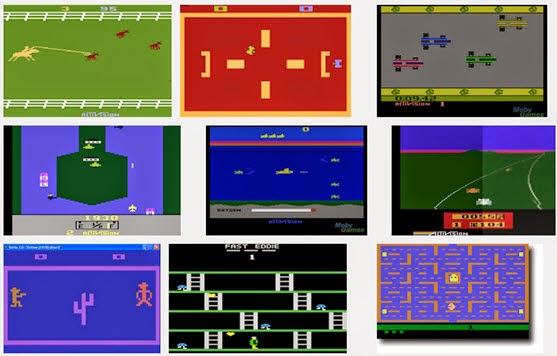
\includegraphics[width=0.6\textwidth]{figures/atari.jpg} 
    \caption{DQN e diferentes jogos Atari.}
    \label{fig:alphago}
\end{figure}	
\end{itemize}
\end{frame}

\begin{frame}{Motivação}
\begin{itemize}
\item
	No mesmo ano, AlphaGo derrotou Lee Sedol, campeão mundial de Go.
\item
	Em 2017, (\cite{AlphaGoZero}) introduziu Alpha Go zero.
	\begin{figure}
	\centering
    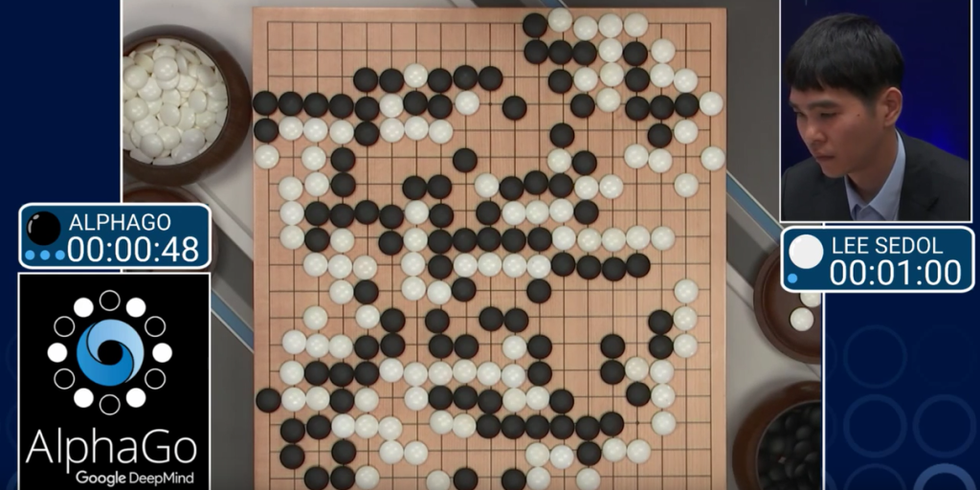
\includegraphics[width=0.6\textwidth]{figures/alphago.png} 
    \caption{AlphaGo contra Lee Sedol.}
    \label{fig:alphago}
\end{figure}
\end{itemize}
\end{frame}

\begin{frame}{Motivação}
\begin{itemize}
\item
	Controle de movimento é um grande desafio para IA.
%	Aprendizado de movimentos reais é uma classe de problemas muito mais difíceis.
\item
	Em 2018, (\cite{deepmimic}) introduziu Deep Mimic.
\item
	%It was able to learn different movements in a simulated scenario.
	Aprendizado de diversos movimentos em ambiente simulado (correr, chutar, acrobacias, etc)
	\begin{figure}
	\centering
    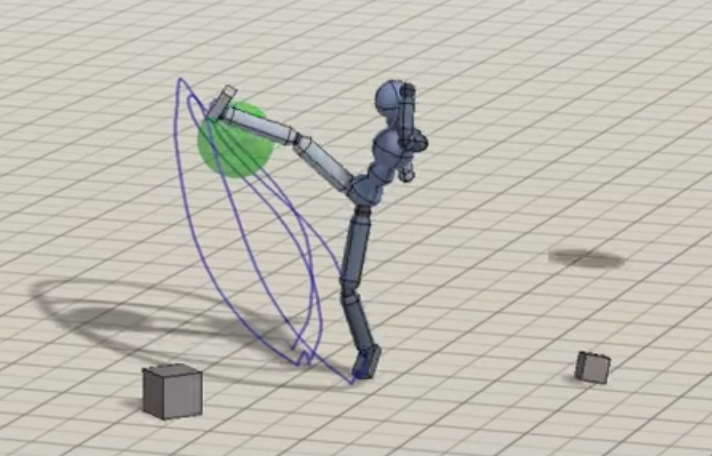
\includegraphics[width=0.5\textwidth]{figures/deepmimic.png} 
    \caption{Humanoid chutando em DeepMimic.}
    \label{fig:alphago}
\end{figure}
\end{itemize}
\end{frame}

\begin{frame}{Motivação}
\begin{itemize}
\item
	RoboCup 3D Soccer Simulation
\begin{figure}[ht]
  	\centering
  	\begin{subfigure}[b]{0.8\textwidth}
              \centering
	 		
\includegraphics[height=0.3\textheight]{figures/RoboCup.png}	
     \end{subfigure}
     
	 \begin{subfigure}[b]{0.45\textwidth}
              \centering
	 		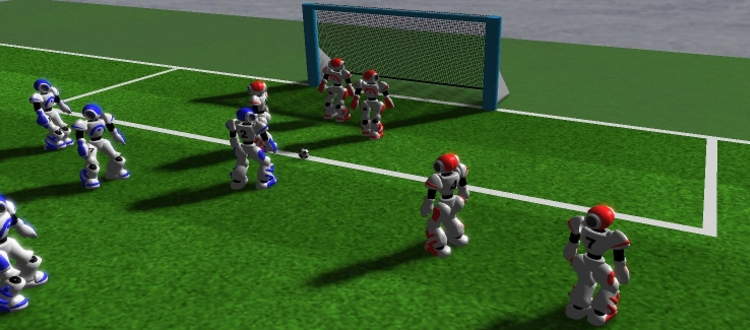
\includegraphics[height=0.3\textheight]{figures/SS3D.png}
	 \end{subfigure}
	     
	 \caption{Símbolo da Robocup e uma partida da liga Soccer 3D.}
	\label{fig:robocup}
\end{figure}	

\end{itemize}
\end{frame}

\begin{frame}{Problema}
\begin{itemize}
\setlength\itemsep{1em}
\item
	Chutar uma bola a uma distância final do agente planejada.
	%Kick the ball towards a planned final distance from the agent.
\item
	%Learn a complete behavior.
	Aprender um comportamento de baixo nível completo.
\item
	Input: estado do agente. Output: sinais de controle para as juntas.
	%Input agent state, output control signals to the joints.
\end{itemize}
\end{frame}

\begin{frame}{Abordagem}
\begin{itemize}
\setlength\itemsep{1em}
\item
	Técnicas recentes de Deep Reinforcement Learning.
	%Modern Deep Reinforcement Learning techniques.
\item
	Inicialmente, aprender por imitação (\cite{deepmimic}).
	%Learn from imitation first \cite{deepmimic}.
\item
	Curriculum learning (\cite{BengioCurrLearning}).
	%Curriculum learning \cite{BengioCurrLearning}.
\item
	Fornecer a distância planejada como entrada da política. Treinar para diversos valores.
	%Input the target distance to the policy NN, train for several values.
\end{itemize}
\end{frame}

\begin{frame}{Revisão Literária}
\begin{itemize}
\setlength\itemsep{1em}
\item
	Técnicas recentes, como DDPG (\cite{DDPG}), TRPO (\cite{TRPO}), PPO (\cite{PPO}).
\item
	Trabalho passado nesse problema: (\cite{abbas}).
\item
	Ainda faz uso de um movimento keyframe. Utilizou CREPS-CMA para aprender $\pi(\theta|s)$.
\item
	(\cite{TGMuzio}) desenvolveu comportamentos de alto nivel para movimentos de drible e roubo de bola no SS3D usando DRL.	
\end{itemize}
\end{frame}

% ================================================================================
\section{Aprendizado por reforço}

\begin{frame}{Introdução ao modelo}
\begin{itemize}
\item
	Interagir com o ambiente, obter recompensas, aprender.
	%Interact with the environment, get rewards, learn.
\begin{figure}[H]
    \centering
    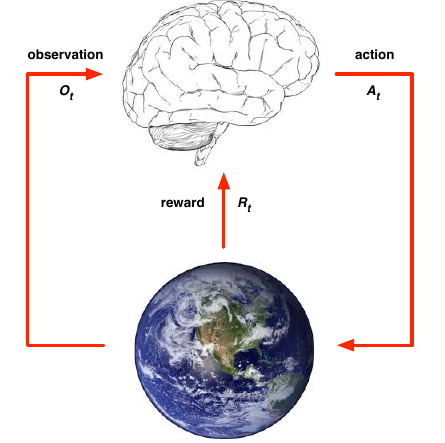
\includegraphics[width=0.4\textwidth]{figures/RL_basic_model.png} 
    \caption{Agente interagindo com o ambiente.}
    \label{fig:RL_basic_model}
\end{figure}
\end{itemize}
\end{frame}

\begin{frame}{Markov Decision Processes}
\begin{itemize}
\item
	Cadeia de Markov $P(S_{t+1} | S_t) = P(S_{t+1} \mid S_1, ..., S_t)$
\item
	Tupla $<\textbf{S}, \textbf{A}, P, R, \gamma>$
	\begin{itemize}
	\item
		$\textbf{S}$ é um conjunto finito de estados que um agente pode assumir.
		%$\textbf{S}$ is a finite set of states the agent can assume in the environment.
	\item
		$\textbf{A}$ é um conjunto finito de ações que um agente pode tomar.
		%$\textbf{A}$ is a finite set of actions the agent can take.
	\item
		$P$ é a função probabilidade de transição para o estado, representado por $P_{ss'}^a = \mathbb{P}[S_{t+1}=s' \mid S_t = s, A_t = a]$.
		%$P$ is a state transition probability function, represented as $P_{ss'}^a = \mathbb{P}[S_{t+1}=s' \mid S_t = s, A_t = a]$
	\item
		$R$ é a função de recompensa imediata, com valor esperado dado por $R_s^a = \mathbb{E}[R_{t+1} \mid S_t = s, A_t = a]$.
		%$R$ is the immediate reward function, with expected value given by $R_s^a = \mathbb{E}[R_{t+1} \mid S_t = s, A_t = a]$
	\item
		$\gamma$ é o fator de disconto, tal que $\gamma \in [0,1]$.
		%$\gamma$ is a discount factor, such that $\gamma \in [0,1]$, used to compute the cumulative total reward.
	\end{itemize}
\end{itemize}
\end{frame}

\begin{frame}{Outros Conceitos}
\begin{itemize}
\setlength\itemsep{1em}
\item
	Retorno total $G_t = R_{t+1} + \gamma R_{t+2} + ... = \sum_{k=0}^{\infty}{\gamma^k R_{t+k+1}}$
\item
	Política $\pi(a \mid s) = \mathbb{P}[A_t=a | S_t=s]$
\item
	State value function $v_{\pi}(s) = \mathbb{E}_{\pi}[G_t \mid S_t = s]$
\item
	Action value function $q_{\pi}(s,a) = \mathbb{E}_{\pi}(G_t \mid S_t = s, A_t = a)$	
\end{itemize}
\end{frame}

\begin{frame}{Algoritmos Clássicos}
\begin{itemize}
\setlength\itemsep{1em}
\item
	Métodos Monte Carlo.
\item
	Temporal-Difference e Sarsa
\item
	Policy Search
\item
	Actor Critic
\item
	(\cite{Sutton1998})
\end{itemize}
\end{frame}

% ================================================================================
%\section{RL Classic algorithms}

%\begin{frame}{Temporal Difference}
%\end{frame}

%\begin{frame}{Policy Search}
%\end{frame}

%\begin{frame}{Actor-Critic}
%\end{frame}

% ================================================================================
\section{Redes Neurais}

\begin{frame}{Motivação}
\begin{itemize}
\item
	Em espaço de ações contínuo, precisamos estimar value functions complexas e não-lineares.
	%In continuous action space, we need to fit complex and non-linear value functions
	\begin{figure}[H]
    \centering
    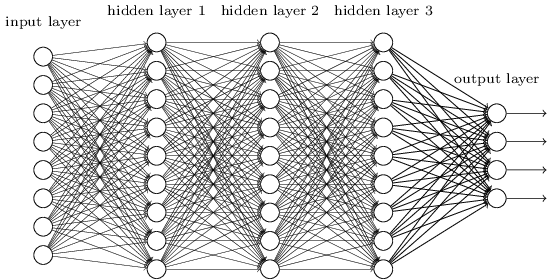
\includegraphics[width=0.6\textwidth]{figures/deep_neural_net.png} 
    \caption{Deep Neural Network.}
    \label{fig:RL_basic_model}
	\end{figure}
\end{itemize}
\end{frame}

\begin{frame}{Métodos}
\begin{itemize}
\item
	Técnicas consagradas.
\begin{figure}[H]
    \centering
    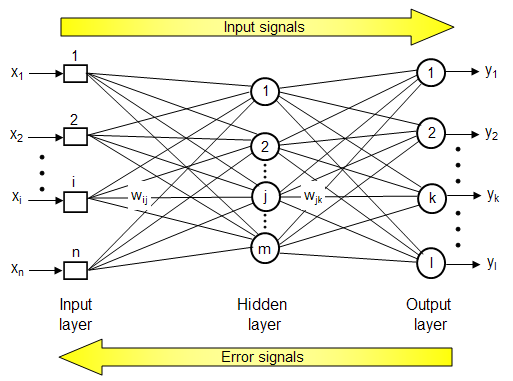
\includegraphics[width=0.45\textwidth]{figures/Feed-Forward-Neural-Network-with-Back-Propagation.png} 
    \caption{Forward and Backward propagation.}
    \label{fig:RL_basic_model}
\end{figure}
\item
	Otimizações: Regularization, RMSprop, Adam Optimizer
\end{itemize}
\end{frame}

%\begin{frame}{Otimizações}
%\end{frame}

% ================================================================================
\section{Deep Reinforcement Learning}

\begin{frame}{TRPO}
\begin{itemize}
\item
	Representa $\pi_{\theta}(a|s)$ como uma distribuição $\mathcal{N}(\mu,\sigma)$. $\mu$ e $\sigma$ output da rede neural.
\item
	Vulnerabilidde ao tamanho do passo de atualização de métodos tradicionais em policy gradient.
	%Vulnerability to the step size in the vanilla policy gradient methods.
\item
	Restringir o tamanho do passo a uma região de confiança
	%Constraining the step size to lie within a trust region.
\begin{equation}
\underset{\theta}{\textrm{maximize }} \mathbb{\hat{E}}_{s_t,a_t \sim \pi_{\theta_{old}} } \left[ \frac{\pi_{\theta}(a_t|s_t)}{
\pi_{\theta_{old}}(a_t|s_t)}\hat{A}_t \right]
\label{eq:TRPO_1}
\end{equation}
\begin{equation}
\textrm{subject to } \mathbb{\hat{E}}_{s_t,a_t \sim \pi_{\theta_{old}} } \left[ KL[\pi_{\theta_{old}},\pi_{\theta}(.|s_t)] \right] \leq \delta
\label{eq:TRPO_2}
\end{equation}
\end{itemize}
\end{frame}

\begin{frame}{PPO}
\begin{itemize}
\item
	Ainda podemos manter essa restrição, mas através de uma implementação mais simples.
	%We can still constrain the step-size, but with a easier implementation.
\item
	Otimização de primeira ordem, com uma função objetivo modificada.
	%First-order optimization, with a modified objective function.
\begin{equation}
r_t(\theta) = \frac{\pi_{\theta}(a_t|s_t)}{\pi_{\theta_{old}}(a_t|s_t)}
\label{eq:def_r_t}
\end{equation}

\begin{equation}
L(\theta) = \mathbb{\hat{E}}_t \left[ min(r_t(\theta)\hat{A}_t, clip(r_t(\theta),1-\epsilon,1+\epsilon)\hat{A}_t) \right]
\label{eq:PPO_objective_function}
\end{equation}
\end{itemize}
\end{frame}

% ================================================================================
\section{Setup e Ferramentas}

\begin{frame}{Ambiente e Ferramentas}
\begin{columns}[T] % align columns
\begin{column}{.5\textwidth}
 \begin{itemize}
 \setlength\itemsep{1em}
  \item Simulador SimSpark (SimSpark 2004)
  \item C++
  \item Python
  \begin{figure}[h!]
   \centering
       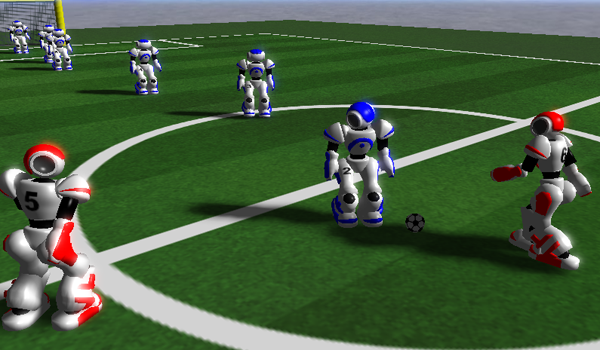
\includegraphics[width=0.8\textwidth]{figures/simspark.png}
 \caption{Simulador SimSpark.}
\end{figure}
 \end{itemize}
\end{column}
\begin{column}{.5\textwidth}
  
  \begin{figure}[h!]
   \centering
       
\includegraphics[width=0.7\textwidth]{figures/tensorflow.png}
 \caption{Logo TensorFlow.}
\end{figure}
  \begin{figure}[h!]
   \centering
       
\includegraphics[width=0.7\textwidth]{figures/openai.png}
 \caption{Logo OpenAI.}
\end{figure}
\end{column}
\end{columns}
\end{frame}

\begin{frame}{Arquitetura}
\begin{itemize}
\item
	Implementada em (\cite{TGMuzio}).
\begin{figure}[h!]
   \centering
       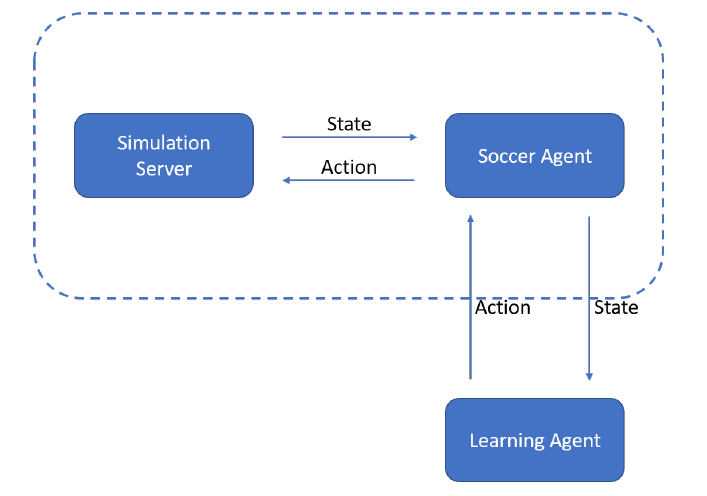
\includegraphics[width=0.6\textwidth]{figures/architecture.png}
\caption{Arquitetura a ser usada.}
\end{figure}
\end{itemize}
\end{frame}

% ================================================================================
\section{Cronograma}

\begin{frame}{Feito}
\begin{itemize}
\item
	Aprender aprendizado supervisionado.
	%Study Supervised Learning.
\item
	Aprender aprendizado por reforço.
	%Study Reinforcement Learning.
\item
	Revisão bibliográfica.
	%Get up-to-date with RL literature.
\item
	Implementar técnicas tradicionais de RL para alguns problemas simples de controle da OpenAI gym.
	%Implement classical RL techniques to some OpenAI gym simple control problems.
\begin{figure}[h!]
   \centering
       
\includegraphics[width=0.3\textwidth]{figures/gym.png}
 \caption{Logo OpenAI Gym.}
\end{figure}
\end{itemize}
\end{frame}

\begin{frame}{Problemas Gym}
\begin{itemize}
\item
	CartPole com Deep Q-Networks.
\begin{figure}[h!]
   \centering
       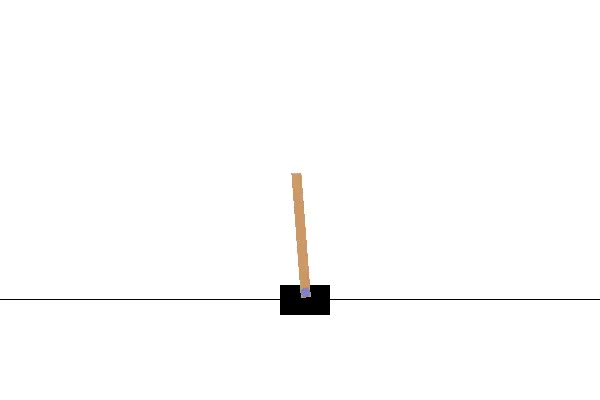
\includegraphics[width=0.35\textwidth]{figures/cartpole.jpg}
 \caption{Cart Pole Gym.}
\end{figure}

\item MountainCar com policy gradient.
\begin{figure}[h!]
   \centering
       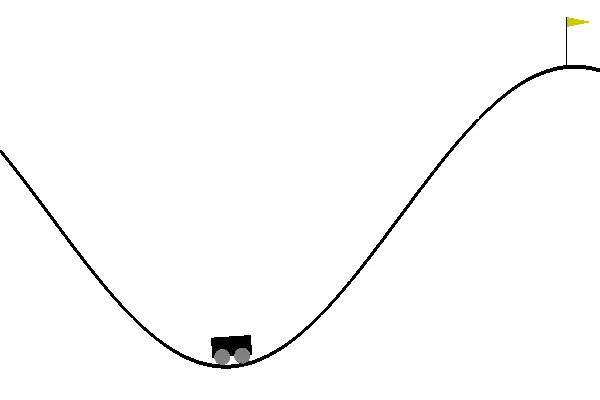
\includegraphics[width=0.35\textwidth]{figures/mountaincar.jpg}
 \caption{Mountain Car Gym.}
\end{figure}

\end{itemize}
\end{frame}

%\begin{frame}{Conclusões}
%\begin{itemize}
%  \item Minha conclusão
% \end{itemize}
%\end{frame}

\begin{frame}{Trabalhos Futuros}
  \begin{itemize}
  \setlength\itemsep{1em}
    \item
    Aprender um behavior que imita o movimento Keyframe atual para o chute.
    %Learn a behavior that imitates the current keyframe for the kick movement.
    \item
    Inputar uma distância fixa para a política e aprender a alcançar essa distância.
    %Input a fixed distance in the policy and learn to reach that distance.
    \item
    %Try to learn for several discrete distances.
    Aprender para várias distâncias num range discreto.
  \end{itemize}
\end{frame}

%\begin{frame}{Agradecimentos}
%\begin{itemize}
%\item Os autores agradecem o suporte da Fundação de Amparo à Pesquisa do Estado de São Paulo -- FAPESP (processo 2016/03647-3).
%\end{itemize}
%\end{frame}

% ================================================================================
\begin{frame}[allowframebreaks]{Bibliografia}
\printbibliography
%\bibliography{references}{}
%\bibliographystyle{plain}
%\bibliography{refs_exemplo}
\end{frame}


% Structuring a talk is a difficult task and the following structure
% may not be suitable. Here are some rules that apply for this
% solution: 

% - Exactly two or three sections (other than the summary).
% - At *most* three subsections per section.
% - Talk about 30s to 2min per frame. So there should be between about
%   15 and 30 frames, all told.

% - A conference audience is likely to know very little of what you
%   are going to talk about. So *simplify*!
% - In a 20min talk, getting the main ideas across is hard
%   enough. Leave out details, even if it means being less precise than
%   you think necessary.
% - If you omit details that are vital to the proof/implementation,
%   just say so once. Everybody will be happy with that.

% \section{Problem Description}
% 
% \subsection{Connectivity Maintenance Approaches}
% \begin{frame}
% 	\begin{itemize}
% 		\item In the literature, there are several strategies for connectivity maintenance in a group of agents
% 		\begin{itemize}
% 			\item \textbf{\alert{Local} Connectivity Maintenance}: once a communication link is active at $t = 0$, it will be active $\forall t > 0$. \emph{Costly}.
% 			\newline
% 			\item \textbf{\alert{Global} Connectivity Maintenance}: maintain a path between any pair of nodes, with possible elimination of redundant links. \emph{More convenient}. 
% 				\begin{itemize} 
% 					\item L. Sabattini, C. Secchi, N. Chopra and A. Gasparri, \textit{Distributed Global Connectivity Maintenance for Multi-Robot Systems}, , AUTOMATICA IT CONGRESS, Benevento, Italy, 2012\newline
% 				\end{itemize}						 
% 		\end{itemize}
% 		
% 		\item When dealing with real systems, supposing instant data transmission is often a too optimistic approach. What is the impact of communication delay in the global connectivity maintenance?
% 	\end{itemize}
% \end{frame}
% 
% \subsection{Background on Graph Theory}
% \begin{frame}
% 	\begin{columns}
% 		\begin{column}{.6\linewidth}
% 			\begin{itemize}
% 				\item $N$ mobile robots: instantaneous communication links modeled as an undirected graph
% 				\item $\mathcal{N}_i$: neighborhood of $i$-th robot
% 				\item $A \in \mathbb{R}^{N \times N}$: adjacency matrix ($a_{ij}>0$ if $j \in \mathcal{N}_i$; $0$ otherwise)
% 				\item $L = D - A$, where $D = \textit{diag}\left( \left\lbrace d_i \right\rbrace\right)$ and $d_i = \sum\limits_{j=1}^{N}a_{ij}$
% 				\item $0 = \lambda_1 \leq \lambda_2 \leq \ldots \leq \lambda_N$ are the eigenvalues of $L$.
% 				\begin{itemize}
% 					\item $\lambda_2 > 0 \leftrightarrow$ the graph is connected: $\lambda_2$ is then defined as the \textbf{algebraic connectivity of the graph}.
% 				\end{itemize}				 
% 			\end{itemize}
% 		\end{column}
% 		\begin{column}{.4\linewidth}
% 			a. \includegraphics[scale=0.10]{figures/t1.png} \\
% 			b. \includegraphics[scale=0.10]{figures/t2.png} \\
% 			c. \includegraphics[scale=0.10]{figures/t3.png}
% 		\end{column}
% 	\end{columns}
% \end{frame}
% 
% 
% \section{Connectivity Maintenance Control Strategies}
% 
% \subsection{Centralized Control Strategy}
% \begin{frame}
% 	\begin{itemize}
% 		\item $\lambda_2$ \textbf{is easily obtained by estimating } $\upsilon_2$
% 	\end{itemize}
% 	
% 	\begin{equation} \label{eq:control_law0}
% 		\dot{p}_i = u_i^c = csch^2(\lambda_2 - \epsilon).\dfrac{\partial{\lambda}_2}{\partial{p}_i}
% 	\end{equation}
% 	
% 	\begin{equation} \label{eq:dlambda2_descentralizado}
% 		\dfrac{\partial{\lambda_2}}{\partial{p_i}} = {\sum\limits_{j \epsilon N_i}-a_{ij}\left( \upsilon_2^i - \upsilon_2^j  \right)^2.\frac{p_i - p_j}{\sigma^2}}
% 	\end{equation}
% 	
% 	\begin{equation}
% 		a_{ij} = \begin{cases}
% 	\ e^{\dfrac{-(\Vert p_i - p_j\Vert)^2}{(2.\sigma^2)}} & , \Vert p_i-p_j \Vert \leq R \\
% 	 0 	 	& , otherwise
% 	\end{cases} 
% 	\end{equation}
% 	
% 	\begin{equation}\label{eq:updatelaw_5}
% 		\begin{alignedat}{2}
% 		& \dot{\tilde{\upsilon}}_2^i = -k_1.z_1^i -k_2.\sum\limits_{j \ \epsilon N_i}a_{ij}.\left(\tilde{\upsilon}_2^i - \tilde{\upsilon}_2^j\right) - k_3.\left(z_2^i-1\right).\tilde{\upsilon}_2^i -k_4.\vert\tilde{\upsilon}_2^i\vert\tilde{\upsilon}_2^i
% 		\end{alignedat}
% 	\end{equation}
% \end{frame}
% 
% \subsection{Decentralized Control Strategy}
% \begin{frame}
% 	\begin{itemize}
% 		\item \textbf{$\lambda_2$ should be \textit{locally estimated}.}
% 	\end{itemize}
% 
% 	\begin{equation} \label{eq:control_law_decentralized}
% 		\dot{p}_i = u_i^c + u_i^d
% 	\end{equation}
% 	
% 	\begin{equation} \label{eq:u^c_final}
% 		u_i^c = csch^2(\lambda_2 - \epsilon).\dfrac{\partial{\tilde{\lambda}}_2}{\partial{p}_i}
% 	\end{equation}
% 
% 	\begin{equation}	\label{eq:lambda2_decentralized}
% 	\tilde{\lambda}_2 = \dfrac{k_3}{k_2}.\left[1 - Ave\left({(\tilde{\upsilon}_2^i)^2   }\right) \right]
% \end{equation}
% 
% 	\begin{itemize}
% 		\item Decentralized Estimation:
% 		\begin{equation}
% 			\dfrac{\partial{\tilde{\lambda}_2}}{\partial{p_i}} = \sum\limits_{j \in \mathcal{N}_i}{ -a_{ij}\left( \tilde{\upsilon}_2^i - \tilde{\upsilon}_2^j\right)^2.\frac{p_i - p_j}{\sigma^2} }
% 		\end{equation}
% 	\end{itemize}
% 	
% 	\begin{center}
% 		\originalsystem
% 	\end{center}
% \end{frame}
% 
% \begin{frame}
% 	\begin{itemize}
% 		\item Formation Control:
% 	\end{itemize}
% 	\begin{equation}
% 		\bar{a}_{ij}\left( \lambda_2^i \right) = \gamma_i.\textit{csch}^2(\lambda_2^i-\bar\epsilon).\frac{1}{\sigma_2}.\left(\tilde{\upsilon}_2^i - \tilde{\upsilon}_2^j \right)^2.a_{ij}
% 	\end{equation}
% 	\begin{equation}
% 		\dot{p} = -\bar{L}.p + u^{d}
% 	\end{equation}
% 
% 	\begin{itemize}
% 		\item Consensus-Based Formation Control: 
% 			\begin{equation}
% 				u^d = -L*p + b_i(p)
% 			\end{equation}
% 			\ \ where
% 
% 			\begin{equation} \label{eq:b_formationcontrol}
% 				b_i(p) = \begin{cases}
% 					\ \sum\limits_{j \epsilon N_i}\left( 1+\bar{a}_{ij}(\lambda_2^i) \right).\left( \bar{p}_i - \bar{p}_j \right) & , \ if \ \lambda_2^i > k.\tilde{\epsilon}  \\
% 	 				\ \sum\limits_{j \epsilon N_i}\left( 1+\bar{a}_{ij}(k.\tilde{\epsilon}) \right).\left( \bar{p}_i - \bar{p}_j \right) &  \ , \ otherwise
% 				\end{cases} 
% 			\end{equation}	
% 	\end{itemize}
% 
% \end{frame}
% 
% \subsection{Decentralized Control Strategy with Communication Delay}
% \begin{frame}
% 	\begin{itemize}
% 		\item Modelling Communication Delay:
% 			\begin{equation}
% 				\upsilon_2^{i^\prime}(t) = \upsilon_2^i(t-\delta)	 \ , \ for \ \delta > 0
% 			\end{equation}					
% 			\begin{equation}
% 				\upsilon_2^{i^\prime} \longrightarrow \lambda_2^{i^\prime}		
% 			\end{equation}
% 		
% 		\item Connectivity estimates error is limited:
% 			\begin{equation}
% 				\vert\lambda_2^{i^\prime} - \lambda_2^\prime\vert \leq \Xi, \forall i = 1, \ldots, N
% 			\end{equation}
% 			\begin{equation}
% 				\vert \lambda_2^{i^\prime} - \tilde{\lambda}_2\vert \leq \Xi^\prime,  \forall i = 1, \ldots, N
% 			\end{equation}
% 		
% 			\begin{center}
% 				\modifiedsystem
% 			\end{center}
% 	\end{itemize}
% \end{frame}
% 
% \begin{frame}
% 	\begin{itemize}
% 		\item Tipically-real agents:
% 			\begin{equation}
% 				u^c \sim 10 \ rad/s
% 			\end{equation}
% 		\item First-order LP Filter:
% 			\begin{equation}
% 				H(s) = \frac{10}{s + 10}
% 			\end{equation}
% 			
% 		\item Cases considered:
% 			\begin{equation}
% 				\delta = 5 \ ms
% 			\end{equation}
% 			\begin{equation}
% 				\delta = 10 \ ms
% 			\end{equation}
% 	\end{itemize}
% \end{frame}
% 
% 
% 
% \section{Results}
% 
% \subsection{Simulation Results}
% \begin{frame}
% 	\begin{itemize}
% 		\item[A.] $\lambda_2$ for $N = 5$ with $\delta = 5 \ ms$
% 		\includegraphics[scale=0.5]{figures/lmbd_2-N5_fail0_delay5E-3_noise0_Nobst150_t5_1sim_Fs10k_lpFilt}
% 	\end{itemize}
% 	
% \end{frame}
% 
% \begin{frame}
% 	\begin{itemize}
% 		\item[B.] $\lambda_2$ for $N = 5$ with $\delta = 10 \ ms$
% 		\includegraphics[scale=0.5]{figures/lmbd_2-N5_fail0_delay1E-2_noise0_Nobst150_t5_1sim_Fs10k_lpFilt}
% 	\end{itemize}
% \end{frame}
% 
% \begin{frame}
% 	\begin{table}[htbp]
% 	\begin{center}
% 		\begin{tabular}{|l|l|l|}
% 			\hline
% 			Measure & A & B \\ \cline{1-3}
% 			$t \ (enter \  obstacle \ set) $ & $0.99 \ s$ & $0.94 \ s$ \\
% 			$t \ (exit \ obstacle \ set)$ & $3.51 \ s$ & $3.97 \ s$ \\
% 			$u^{c^{min}} (obstacles \ crossing)$ & $0.05$ & $0$  \\
% 			$u^{c^{max}} (obstacles \ crossing)$ & $0.84$ & $0$ \\
% 			min. $\lambda_2^i \ (t=5s)$ & $3.55$ & $-18.6$ \\
% 			max. $\lambda_2^i \ (t=5s)$ & $3.55$ & $11.0$ \\
% 			\cline{1-3}
% 		\end{tabular}			
% 	\end{center}
% 	\end{table}
% \end{frame}
% 
% \subsection{Conclusions and Future Work}
% \begin{frame}
% 	\begin{itemize}
% 		\item $\lambda_2 > 0$ only for $\delta \approx 0$
% 		\newline
% 		\newline
% 		\item $\lambda_2^i$ cannot be trusted if $\delta > 0$, as $u^c$ is unable to prevent $\lambda_2 = 0$
% 		\newline
% 		\newline
% 		\item As \textit{Future Work}, one can relate the analysis of the algorithms described in [Secchi, 2012] and [Secchi, 2013], that propose a solution to deal with time delay in the communication between agents.
% 	\end{itemize}
% 	
% \end{frame}
% 
% \begin{frame}
% 	\begin{center}
% 		\emph{Thank you!}
% 	\end{center} 
% \end{frame}

\end{document}


